\fancychapter{Implementation of a Rapport Agent}
\label{chap:proposedapproach}

The following sections describe the implementation of the rapport model, as well as the framework that eases the development of rapport agents by both technical and non-technical researchers. The framework is built on top of the \ac{SERA} ecosystem as it provides most of the tools to translate high-level intentions into actions that can be executed by either virtual or robotic agents such \ac{EMYS} (Figure~\ref{fig:robots:EMYS2}) and NAO (Figure~\ref{fig:robots:NAO2}). The latter robot is the chosen embodiment to test the developed rapport agent.

Following this, the framework has the following goals:
\begin{enumerate}
	\item Implement the rapport model described in Chapter~\ref{chap:rapportModel};
	\item Promote re-usage of interaction strategies among different agents and \ac{HRI} scenarios;
	\item Provide non-technical researchers with the tools to customise the agent's behaviour;
	\item Provide technical researchers with the tools to develop additional rapport strategies without hindering the performance of the existing ones;	
	\item Maintain compatibility with current agents developed using the \ac{SERA} ecosystem.
\end{enumerate}

%TODO verificar following... depiction

\begin{figure}[ht]
	\centering
	\begin{minipage}[b]{.4\textwidth}
		\centering
		\frame{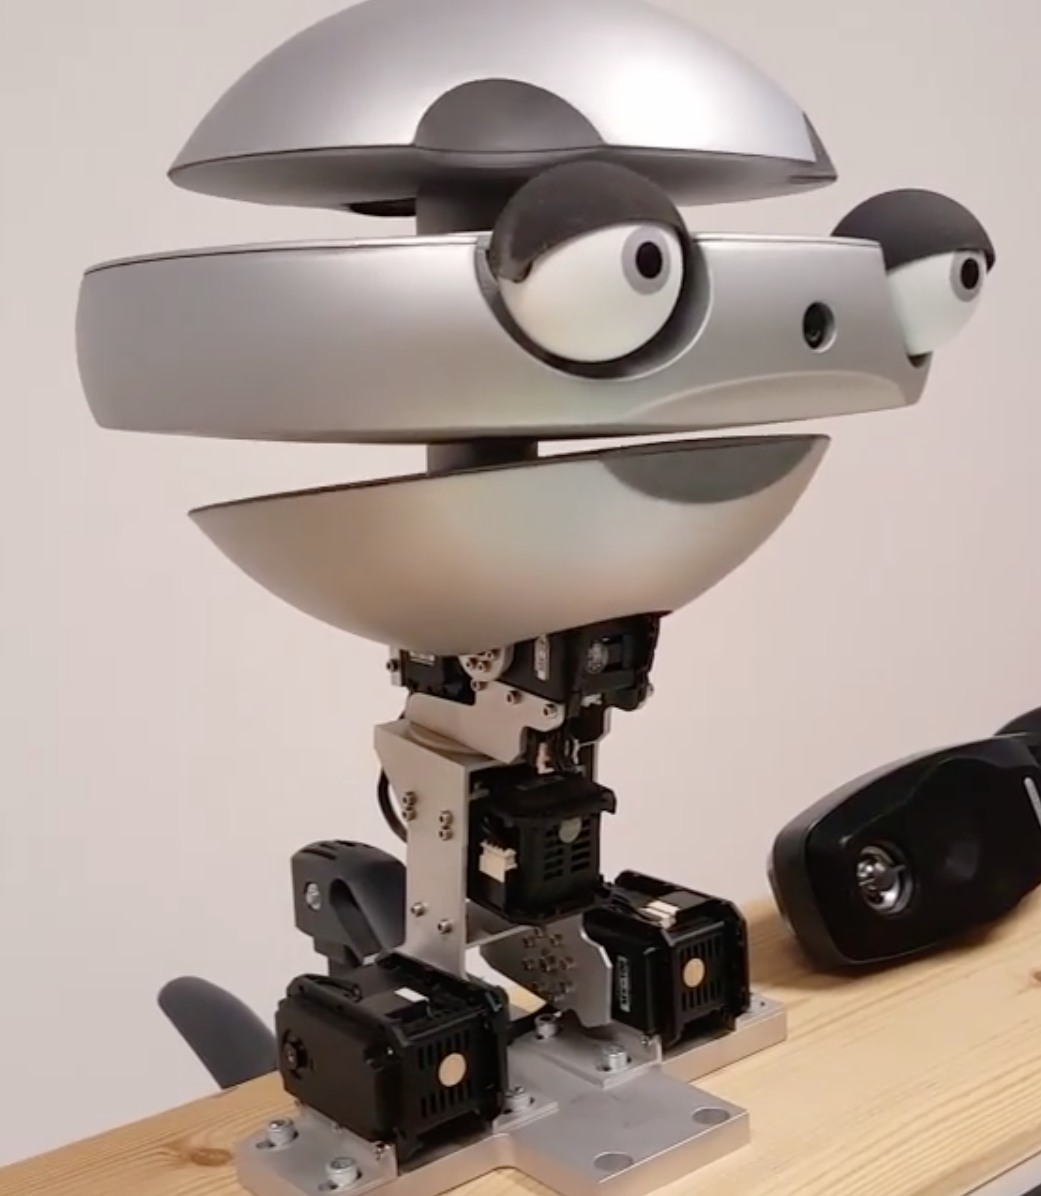
\includegraphics[width=0.4\textwidth]{images/emys.png}}
		\caption{\ac{EMYS} robot.}
		\label{fig:robots:EMYS2}
	\end{minipage}
%	\hfill
	\begin{minipage}[b]{.4\textwidth}
		\centering
		\frame{
\includegraphics[width=0.55\textwidth]{images/NAO_Robot.JPG}}
		\caption{NAO robot.}
		\label{fig:robots:NAO2}
	\end{minipage}
\end{figure}



\section{\acf{SERA}: Features and Limitations}
\label{sub:sera:features_limitations}

Revisiting Section~\ref{sub:sec:SERA}, the \ac{SERA} framework is built on top of \textit{Thalamus} network, where \textit{Thalamus} clients communicate with one another through network messages. For example, \textit{Effector Thalamus} clients, in order to change agent's behaviour have to contact \textit{Skene} that processes and redirects the request to the most suitable clients: \textit{Nutty Tracks} for animations and \textit{Speech Server} for utterances. In addition, it has a finer control over the agent's action, able to, for example, causing delays or generate idle behaviour.

\ac{SERA} already assures a decoupled design for agents by using different \textit{Thalamus} clients with different responsibilities, cooperating with one another through well-defined \textit{Thalamus} network messages. Moreover, there is already support for interrupting ongoing actions, however, we need to assess how well \textit{SERA} agents are capable to quickly adapt to the dyadic state of the interaction. To this end, we ran the tests described in the following paragraphs.

In the first test, we measured the response speed between requesting an action and its execution. Following Figure~\ref{fig:solution:sera_simple_message_delay}, an \textit{Effector} \textit{Thalamus} client (in the role of a potential rapport strategy) sends an utterance request to the \textit{Skene} client. The request is dispatched and processed in \textit{Skene} and redirected to the \textit{Speech Server} which executes the desired utterance. However, each network message has to pass through \textit{Thalamus} so that it can redirect the messages to the target clients in the network. The test was successful although:

\begin{itemize}
	\item If a speech request arrives while there is one in execution, the \textit{Speech Server} executes them sequentially which can have undesired effects. For example, an \textit{Effector} may request utterance twice as a reaction to the external environment making the \textit{Speech Server} run them both twice, one after another, regardless of their duration;
	\item There is a noticeable (less than a second) delay between the requests and the effects, as requests pass firstly through \textit{Skene}, \textit{Thalamus} and finally, either \textit{Nutty Tracks} or \textit{Speech Server} (Figure~\ref{fig:solution:sera_simple_message_delay} and~\ref{fig:solution:sera_complex_message_delay}).
\end{itemize}

\begin{figure}[H]
	\centering
	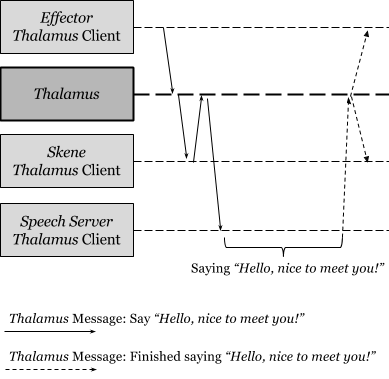
\includegraphics[width=0.45\textwidth]{images/SERA_SimpleTest.png}	
	\caption{\textit{Thalamus} network messages sent when attempting to execute a vocalisation.}
	\label{fig:solution:sera_simple_message_delay}
\end{figure}

In the second test, we extended the first test to examine the behaviour when interrupting actions (Figure~\ref{fig:solution:sera_complex_message_delay}). The sender requests an utterance to be executed, then interrupts it while it is still in execution. This test was not successful as there was a substantial delay between requesting the interruption and the effect ($\approx$ 3 seconds average in 10 tests).

\subsection*{Discussion}

We repeated the tests described in the previous section with animations instead of utterances but the results were identical. We strongly believe that the results are affected by the network nature of \ac{SERA}. When sending the messages directly from the \textit{Skene}'s \ac{GUI}, the delays were substantial shorter, reduced to less than a second, compared to the previous 3 seconds when sending from a separate client to \textit{Skene} as described in Figure~\ref{fig:solution:sera_simple_message_delay} and Figure~\ref{fig:solution:sera_complex_message_delay}.

To sum up, to accomplish our goals, taking into account \textit{Skene}'s capabilities and the tests previously described, the framework needs to:
\begin{itemize}
	\item Reduce the number of network messages that pass through the network, in order to reduce the latency between the requests and the effects, without breaking compatibility with current agents;
	\item Distribute \textit{Skene} responsibilities to different independent components in order to promote modularisation, and give the researchers the ability to customise the agent's behaviour more easily.
\end{itemize}


\begin{figure}[H]
	\centering
	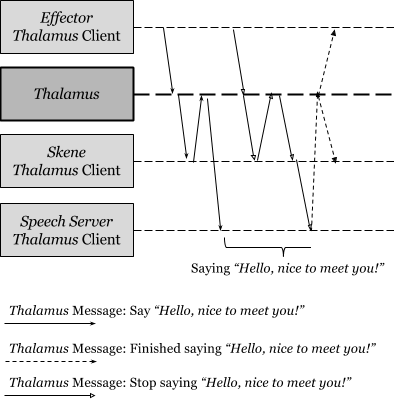
\includegraphics[width=0.45\textwidth]{images/SERA_DelayTest.png}
	\caption{\textit{Thalamus} network messages sent when attempting to execute and interrupt a vocalisation.}
	\label{fig:solution:sera_complex_message_delay}
\end{figure}

\section{Architecture Overview}

The following sections describe the framework that builds the foundations to design rapport agents using a plugin-based paradigm that takes into account the current limitations of the \ac{SERA} framework, and the rapport model detailed in Chapter~\ref{chap:rapportModel}. In order to tackle the delay between the requests and the effect (as described in Section~\ref{sub:sera:features_limitations}), the framework limits the number of network messages by communicating internally though regular method calls and events.

Following Figure~\ref{fig:rapport:archicture}, the framework contains the following elements:
\begin{itemize}
	\item \textbf{\textit{Effector Plugins}}: propose actions and enables/disables plugins;
	\item \textbf{\textit{Perceiver Plugins}}: perceive the external world and informs the interested plugins;
	\item \textbf{\textit{Utility Plugins}}: general purpose plugins that can be used to, for example, store the dyadic state of the interaction;
	\item \textbf{\textit{Rapport Controller}}: manages plugins' lifecycle, link plugin, and has the same responsibilities as the rapport model's \textit{Rapport Controller} described in Section~\ref{sec:rapportController} in Chapter~\ref{chap:rapportModel};
	\item \textbf{\textit{Thalamus Connection}}: bridges the system with \ac{SERA}, sending and receiving \textit{Thalamus} messages.
\end{itemize}

\begin{figure}[H]
	\centering
	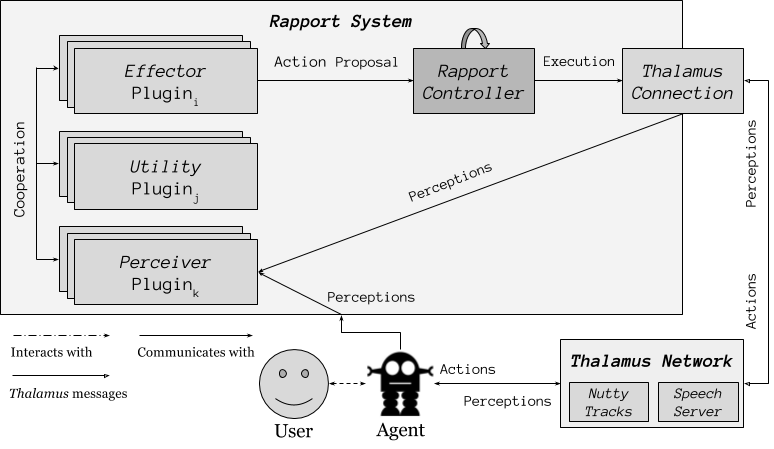
\includegraphics[width=0.9\textwidth]{images/RapportControllerArchitectureOverview.png}
	\caption{Schematic representation of the framework that implements the rapport model.}
	\label{fig:rapport:archicture}
\end{figure}

Following the same Figure~\ref{fig:rapport:archicture}, there are five types of connections:
\begin{itemize}
	\item \textbf{Perceptions}: perceptual information;
	\item \textbf{Actions}: decisive messages that trigger animations or utterances;
	\item \textbf{Action Proposal}: requests sent by \textit{Effector Plugins} that are managed by the \textit{Rapport Controller};
	\item \textbf{Execution}: set of actions triggered periodically by the \textit{Rapport Controller} - execution, interruptions or replacement according to the action proposals' stage;
	\item \textbf{Cooperation}: communication between plugins. For example, \textit{Effectors} use \textit{Perceivers} to read perceptual information and may use \textit{Utility} plugins to consult the interaction history.
\end{itemize}





\section{Rapport Controller}
\label{sec:rapportController2}

In addition to managing the agent's actions as described in the rapport model (Chapter~\ref{chap:rapportModel}), the \textit{Rapport Controller} has the following responsibilities:
\begin{itemize}
	\item Load and manage the lifecycle of the plugins;
	\item Link different plugins;
	\item Provide mechanisms to debug the proposed actions.
\end{itemize}

In the following sections, the document described how the above goals are satisfied by the developed system as well as how it aids technical and non-technical researchers the development of additional behavioural strategies, either through the development of custom plugins (Section~\ref{sec:plugins}), through customisation of specific parameters (Section~\ref{sec:plugins}), or through the definition of behaviour using markup text (Section~\ref{sub:sec:agentActionsManager}).

\subsection{Plugins Lifecycle}
\label{sub:sec:pluginLifecycle}

At the startup, the \textit{Rapport Controller} loads the available plugins from a user-selected folder (each plugin is a dynamically linked library loaded in runtime). They are all enabled by default unless specified otherwise through the configuration file that can be accessed using the controller's \ac{GUI} (Figure~\ref{fig:pluginList}). During this process, following Figure~\ref{fig:pluginLifecycle}, each plugin follows a two-step initialisation:

\begin{enumerate}
	\item \textbf{Initialisation}: initialise internal variables;
	\item \textbf{Retrieve Dependencies}: retrieve plugins that it depends on (e.g., \textit{Effectors} typically requires \textit{Perceivers}). As long as the plugin is enabled, it can be used by its peers.
\end{enumerate}

\begin{figure}[H]
	\centering
	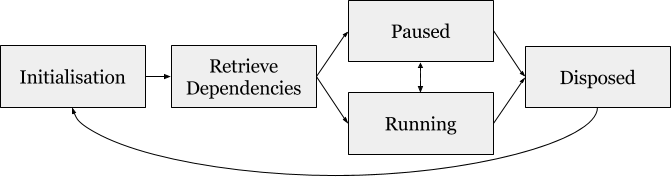
\includegraphics[width=0.7\textwidth]{images/PluginsLifecycle.png}
	\caption{\textit{Rapport Controller}'s plugin's lifecycle.}
	\label{fig:pluginLifecycle}
\end{figure}

After initialisation, the plugins can be either running or paused depending on the state of the \textit{Rapport Controller}. If the controller is running, then \textit{Perceivers} capture external world stimuli and notify the \textit{Effectors} which will attempt to modify the agent's behaviour concurrently by proposing actions asynchronously to the \textit{Rapport Controller} (perceptions events are sent asynchronously but \textit{Effectors} may pool the state of the interaction). The list of active plugins may be changed, either manually by the researcher using the provided \ac{GUI} (Figure~\ref{fig:pluginList}), either automatically by an \textit{Effector} plugin. In any case, in the case of an error in any state transition, the responsible plugin is automatically deactivated and disposed of without escalating to a sudden application crash. Finally, if an error occurs, the researcher is notified with the complete description of the fault.

\begin{figure}[H]
	\centering
	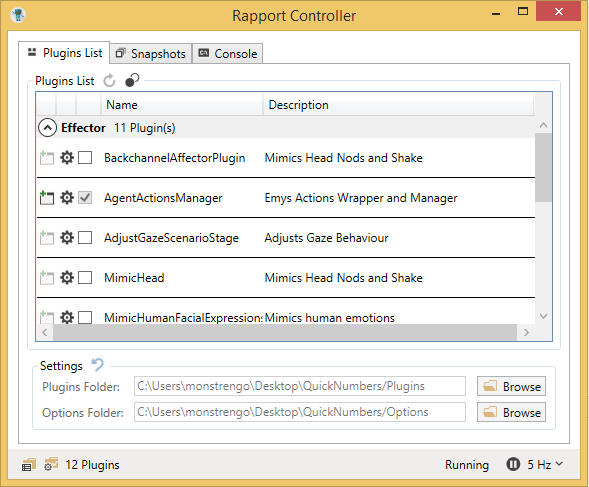
\includegraphics[width=0.6\textwidth]{images/PluginsList.png}
	\caption{\ac{GUI} representation of the list of available plugins.}
	\label{fig:pluginList}
\end{figure}

\subsection{Managing Actions}
\label{sub:sec:managingActions}

The \textit{Rapport Controller} manages action proposals as described in Section~\ref{sec:rapportController} in Chapter~\ref{chap:rapportModel}. However, in addition to the elements of action proposal quintuple $A=<G,P,E,I,T>$, the controller stores the following information:
\begin{itemize}
	\item \textbf{Status}: \textit{pending}, \textit{executing}, \textit{executed} or \textit{interrupted};
	\item \textbf{Starting time}: when the action has started executing;
	\item \textbf{\textit{Thalamus} identifier}: to monitor when actions have finished by monitoring the \textit{Thalamus} messages sent by \textit{Nutty Tracks} and \textit{Speech Server}.
\end{itemize}

The status field is required to manage the state of each action proposal. For example, following Figure~\ref{fig:actionProposalStatus}, an action proposal is only executed (using execution description $E$) as long as its previous state was \textit{pending} and, only then it can be interrupted (using the interruption description $I$). In the absence of the \textit{Thalamus} identifier, we could not flag the actions has executed, making them transition automatically to the \textit{interrupted} state. Furthermore, the controller's default frequency is 10Hz, i.e., the action proposals are analysed 10 times per second.

\begin{figure}[H]
	\centering
	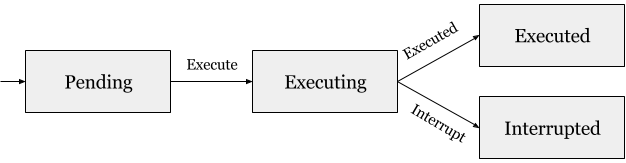
\includegraphics[width=0.6\textwidth]{images/ActionProposalCycle.png}
	\caption{Action Proposal available states and the corresponding transition graph.}
	\label{fig:actionProposalStatus}
\end{figure}

The execution and the interruption descriptions of the action proposal ($E$ and $I$, respectively) are self-contained functions specified by the researcher, therefore they can contain additional logic that is only processed when transitioning to the \textit{executing} state or to the \textit{interrupted} state, respectively. However, in order to change the agent's behaviour, they have to send the required \textit{Thalamus} messages: \textit{Speech Server} to produce utterances or \textit{Nutty Tracks} to trigger animations.

To sum up, the \textit{Effector Plugins} propose actions specifying its priority, how it should be executed, and can additionally specify how the action can be interrupted. The researcher can use the provided \ac{GUI} to debug the proposals as illustrated in Figure~\ref{fig:controllerSnapshots}. Above all, pilots are required to specify the optimal configuration of actions and their priority so that the agent's behaviour satisfies the scenario goals. 

\begin{figure}[H]
	\centering
	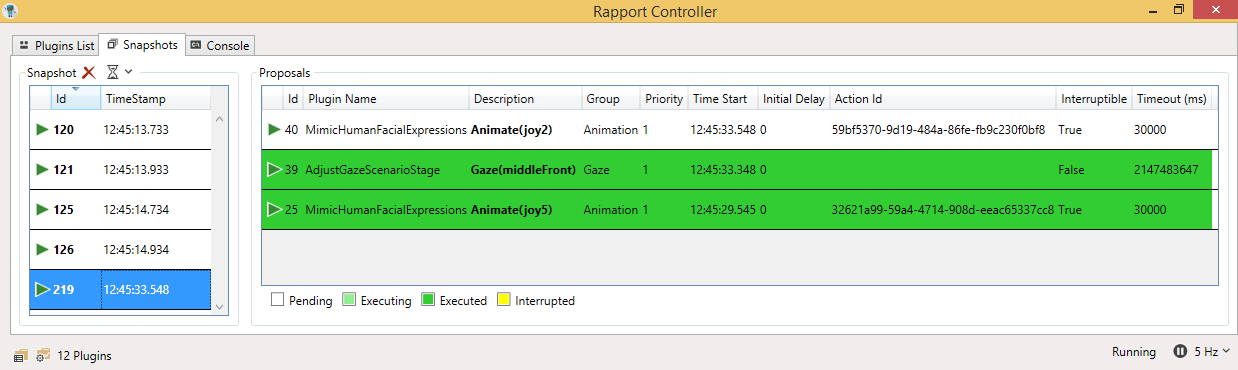
\includegraphics[width=\textwidth]{images/ScreenshotSnapshots.png}
	\caption{\ac{GUI} representation of the snapshots retrieved periodically by the \textit{Rapport Controller}.}
	\label{fig:controllerSnapshots}
\end{figure}
\section{Plugins}
\label{sec:plugins}

There are three types of plugins: \textit{Effectors}, \textit{Perceivers}, and \textit{Utility}. Their responsibility is to propose actions, to receive external world stimuli and support its peers, respectively. For the developers, the \textit{Effectors} are the only ones capable of proposing actions and changing the status of other plugins, the remaining types are identical, only differing by its name.

Furthermore, one of the goals of this project is to provide the developers with the flexibility to reuse their components on different scenarios with little to no additional effort. For this purpose, researchers only need to focus on the essentials components of the plugin as the system already provides the tools to handle, for example, optional \ac{GUI} and, more importantly, configuration files to change the rapport \textit{Effectors}' parameters specified throughout Chapter~\ref{chap:rapportModel}. The configuration file is a \ac{XML} document that is loaded during the plugin's initialisation, and can be modified afterwards (and saved) in runtime by accessing the configuration file (Listing~\ref{lst:facialExpressionsSettings} in Appendix B) by clicking on the settings icon depicted on each row in Figure~\ref{fig:pluginList}. The major advantage is that the developer does not need to recompile the plugins just to make this change. Lastly, the plugin's \ac{GUI} can be opened from the controller's user interface (Figure~\ref{fig:pluginList}). An \textit{Effector} that mimics facial expression is listed in Listing~\ref{lst:facialExpressionsSourceCode} in Appendix C.

\subsection{Effector}
\label{sub:sec:effectorPlugin}

%One could argue that another \textit{Effector} could lock the Face Action Group with an empty action with higher priority, however, this is an elaborate solution that adds unnecessary complexity to the system. An easier solution is to, track the current gaze target, and deactivate and enable the \textit{Effectors} that rely on direct eye contact.

The main task of the \textit{Effectors} was described previously in Section~\ref{sub:sec:managingActions}. However, during development, we identified a key use case that greatly impacts interactions. During the development of the scenario described in Chapter~\ref{chap:userstudies}, we identified that it would be helpful if we could deactivate and enable plugins in runtime, allowing specific rapport strategies to only affect discrete sections of the scenario. For example, deactivate idle behaviour if the agent is attentive to the task. This mechanism should be handled by a separate higher-level plugin that maps the agent's state to the list of enabled rapport strategies, leaving the essential to the \textit{Effector}.

Another key issue that emerged was internal conflict within the \textit{Effector} where it would interrupt himself repeatedly. For example, during the initial stages, the behavioural mimicry rapport \textit{Effectors} from the rapport model, described in Section~\ref{sub:model_Coordination}, were interrupting themselves regularly because the \textit{Perceiver} was continuously notifying them. To solve this issue, we added, transparently to the developer, a mechanism to track internally the proposed actions, and an additional parameter that specifies the minimum interval of time between action proposals. The researcher can choose on of the following levels:

\begin{itemize}
	\item \textbf{Unrestricted}: the \textit{Effector} must explicitly manage its proposed actions;
	\item \textbf{One Action Globally}: the \textit{Effector} cannot interrupt itself unless with a proposal with higher priority;
	\item \textbf{One Action Per Group}: same as \textit{One Action Globally} but granulated to the \textit{Group}.
\end{itemize}

In short, the task greatly influences how the different plugins will have to cooperate with one another in order to satisfy the behavioural goals of the interaction. For example, it is crucial to properly define the priority of the action proposals as it is fundamental to manage which actions will be triggered and which actions will be interrupted at any given time. To recall the reader, behaviours triggered by singular events should have higher priorities than events that happen commonly. For example, a surprise emotion (an emotion typically raised by an unexpected sudden event) should have higher priority than, for example, a happy facial expression that is at the moment mimicking the interactional partner emotion.

\subsection{Agent Actions Manager}
\label{sub:sec:agentActionsManager}

%Mencionar que é este o plugin que tem a Thalamus Connection para executar acções

Agent Actions Manager is a \textit{Utility} plugin with the following goals:
\begin{itemize}
	\item Monitors agent's actions to notify the \textit{Rapport Controller};
	\item Provide convenient wrappers for common action proposals, describing both execution and interruption descriptions ($E$ and $I$): animations, utterances, vocalisations, sounds, head nods, head shakes, and gaze;
	\item Provide non-technical researchers with the tools to change the agent's behaviour given the dyadic state of the interaction, without worrying about implementation details.
\end{itemize}

The first objective is achieved by monitoring the messages that both \textit{Speech Server} and \textit{Nutty Tracks} send to the \textit{Thalamus Network}, and compare the actions' identifiers with the stored ones. They both notify whenever their actions have started or have finished, therefore this plugin just monitors those messages containing the action \texttt{id} and redirects them to the \textit{Rapport Controller}. The second objective aims to reduce the amount of code required to specify common action proposals. Therefore, the \textit{Effectors}, in order to use the provided tools, have to request the \textit{Rapport Controller}, the Agent Actions Manager \textit{Utility} plugin during the \textit{Initialise dependencies} stage of the initialisation (Figure~\ref{fig:pluginLifecycle} in Section~\ref{sub:sec:pluginLifecycle}).

\begin{figure}[H]
	\centering
	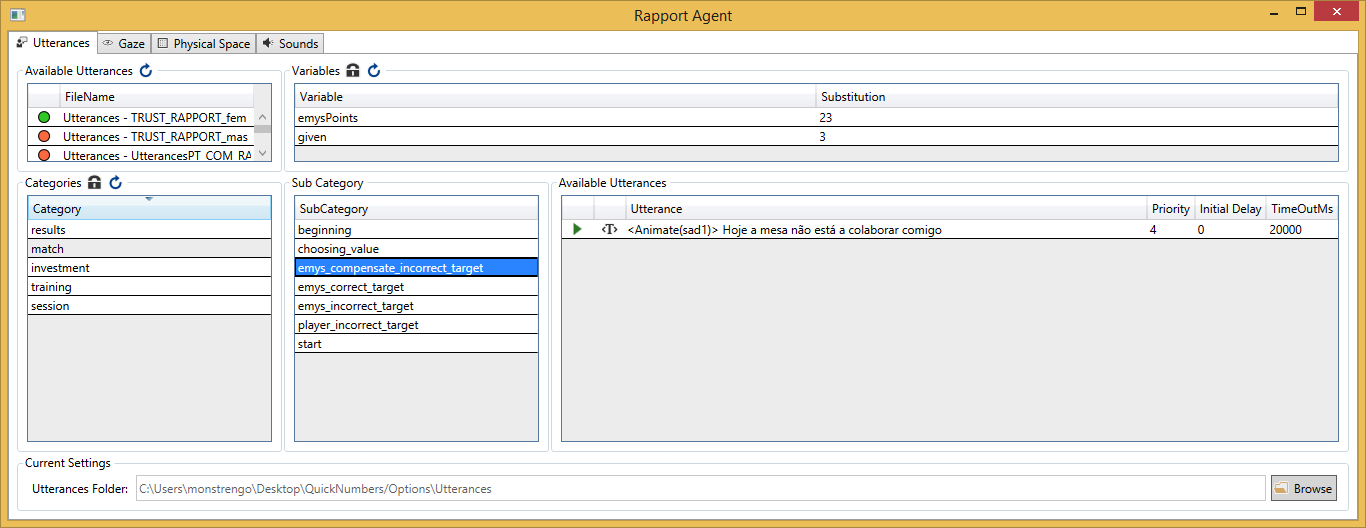
\includegraphics[width=\textwidth]{images/ScreenshotAgentsManager.png}
	\caption{\ac{GUI} representation of the Agent Action Manager \textit{Utility} plugin.}
	\label{fig:agentActionsManagerScreenshot}
\end{figure}

To accomplish the last goal, the Agent Actions Manager \textit{Utility} plugin, similar to \textit{Skene}, provides a \ac{GUI} that provides non-technical researchers with the tools to collaboratively change the agent's behavioural rules or utterances (Figure~\ref{fig:agentActionsManagerScreenshot}). However, these utterances take advantage of the prioritisation mechanism defined in the rapport model in Chapter~\ref{chap:rapportModel}. For this purpose, following Expression~\ref{eq:behaviour} and Table~\ref{fig:extended:utterances}, researchers can provide the following optional parameters: priority, delay, and timeout. These parameters will default to, the utterance priority, 0 and the utterance's timeout, respectively. 

\begin{equation}
	<action(arg_1, arg_2, ..., arg_n, [priority], [delay], [timeout])>
	\label{eq:behaviour}
\end{equation}

Similar to \textit{Skene}, the set of utterances can be imported from a \ac{CSV} file (using the format specified in Appendix D) and edited directly in the \ac{GUI}. Moreover, the developer may specify substitution variables by adding $|Variable|$ to the content of the utterance. The values of these substitution variables can be defined in the \ac{GUI} or in runtime by the \textit{Effectors}. If there are multiple variables with the same identifier, the ones provided by the \textit{Effector} will override the ones specified in the \ac{GUI}. Lastly, if there are multiple utterances for the same category and subcategory, only one is selected randomly as long as it was not selected in the past.

\begin{table}[H]
	\centering
	\begin{tabular}{|l|l|l|l|l|l|}
	\hline
	\multicolumn{1}{|c|}{\textbf{Category}} & \multicolumn{1}{c|}{\textbf{Subcategory}} & \textbf{Utterance}                                                                                      & \textbf{Priority} & \textbf{Delay (ms)} & \textbf{Timeout (ms)} \\ \hline	
	intro & greet & \specialcell{Hi $|$\textit{Name}$|$!$<$gaze(person)$>$} & 2 & 0 & 30000 \\ \hline
	game & score & \specialcell{Yey!$<$Animate(surprise2,3)$>$} & 2 & 0 & 30000 \\ \hline
	game & results & \specialcell{Managed $|$\texttt{Points}$|$!\\$<$gaze(person,3,500,5000)$>$} & 2 & 0 & 30000 \\ \hline
	end & ending & \specialcell{Thank you for your participation!\\$<$animate(happy4,4,1000)$>$} & 3 & 0 & 30000 \\ \hline		
	\end{tabular}
	\caption{Set of utterances compatible with the framework. Set of utterances compatible with \acf{SERA}. Actions are delimited by $<$ and $>$, and substitution variables by $|$.}
	\label{fig:extended:utterances}
\end{table}




%The \ac{GUI} (Figure~\ref{fig:agentActionsManagerScreenshot}) was done from scratch as the \textit{Rapport Controller} uses a more recent technology, \ac{WPF}.
\section{Rapport \textit{Effectors} Implementation}
\label{sec:rapportStrategies}

The following section describes the most relevant implementation details of the rapport \textit{Effectors} of the model detailed in Chapter~\ref{chap:rapportModel}. As denoted in Sections~\ref{sub:model_positivity}, \ref{sub:model_Coordination}, and \ref{sec:mutual_attentionModel}, the rapport strategies have to be parametrisable, so that researchers may adapt the model to any agent embodiment or \ac{HRI} scenario. 

The Positivity rapport \textit{Effector} (that satisfies the ``Stimulate positivity'' goal) and the ``Adhere to Social Norms'' goal are implemented by triggering utterances given the perceptual information of the scenario. Finally, The \textit{Effectors} were implemented and tested using robot \ac{EMYS} (Figure~\ref{fig:robots:EMYS2}).


%TODO referir que a positivity e o adhere to social norms são implementados scenario based

%In the following sections we will describe the supporting technologies, \ac{SSI}~\cite{Wagner2013}, SHORE~\cite{Ruf2011}, and GRETA~\cite{Niewiadomski2009} in Section~\ref{sec:supportingTechnologies}, followed by a brief description of the \textit{Effectors} described above.

%Most of all, in order to build rapport more effectively, one should take into consideration if the above-mentioned strategies fit the study scenario, and if they are adequate to the person the agent is interacting with (e.g., introvert and extrovert people should be handled differently~\cite{Andrist2015}). This aspect is more relevant for enhancing positivity which is mostly built either through vocal interactions or through gestures. For this purpose, in order to build positivity, the developer must build their own \textit{Effector} or \textit{Effectors}.



% Bull1981, Baxter2014
% Impact on users behaviour
%Buschmeier2011, Zhao2014, Reidsma2011, Gratch2006, Mutlu2006, Andrist2015, Stanton2014,


\subsection{Supporting Technologies}
\label{sec:supportingTechnologies}

Revisiting the rapport model described throughout Chapter~\ref{chap:rapportModel}, the rapport \textit{Effectors} require the following perceptual capabilities:
\begin{itemize}
	\item Monitor the interaction activity, for the Positivity \textit{Effectors}.
	\item Identify human emotions, and head-gestures for the behavioural mimicry \textit{Effectors};
	\item Identify speech disfluencies (Figures~\ref{fig:lowering} to \ref{fig:risingLowering}) for the backchannel \textit{Effector};
	\item Identify the user's gender and monitor the current state of the interaction, for the Mutual-Gaze \textit{Effector};
\end{itemize}

Following Figure~\ref{fig:SupportingTechnologiesOverview}, the system uses \ac{SSI}~\footnote{\url{http://hcm-lab.de/projects/ssi/}} to recognise social-signals in real-time from microphones and video feeds~\cite{Wagner2013}. \ac{SSI} uses SHORE~\cite{Ruf2011} and openSMILE~\cite{Eyben:2013:RDO:2502081.2502224} to recognise emotions, and extract prosody features, respectively. For example, \ac{SSI} identifies head-gestures using a Kinect Camera, and SHORE outputs the different emotion intensities given the video feed. Finally, \ac{SSI} periodically collects and sends the perceptual information in \ac{XML} format through network messages to other processes using ActiveMQ~\footnote{\url{http://activemq.apache.org/}}, specifically GRETA\textsuperscript{PP}.

\begin{figure}[H]
	\centering
	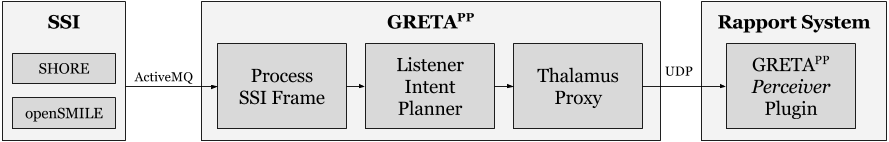
\includegraphics[width=0.95\textwidth]{images/SupportingTechnologiesOverview.png}
	\caption{Schematic representation of the components that supports the rapport model.}
	\label{fig:SupportingTechnologiesOverview}
\end{figure}

GRETA\textsuperscript{PP} is a variation of the GRETA system~\cite{Niewiadomski2009} that uses only the  \textit{Listener Intention Planner} component of the original GRETA (Figure~\ref{fig:GretaOriginal}), as we are not interested in the remaining components for the scope of this thesis. In short, GRETA\textsuperscript{PP} attempts to match the perceptual information to the first behavioural rule defined in a configuration file loaded at launch as exampled in Listing~\ref{lst:exampleGretaRule}. In the case of a match, the system might output a response signal given the response probability specified by the same rule. The original set of rules was reduced, as they were tailored for a virtual agent with different capabilities than the robot \ac{EMYS}, for example, the virtual agent is capable of moving his eyebrows and specific lip positions. Finally, taking advantage that GRETA is already integrated with \ac{SSI}, we adapted \ac{SSI} and GRETA\textsuperscript{PP} to redirect head gestures and facial expressions perceptual information to our system. It is important to mention that there is a slight delay beginning from \ac{SSI} and ending in the \textit{Perceiver}, and that only the emotion with the highest intensity is sent. The major bottleneck of the system relies on \ac{SSI} itself which is resource intensive and, in order to be able to test the system, the refresh rate had to be reduced to 5Hz which is half the default value.


\begin{lstlisting}[caption={One of the backchannels rules used GRETA and GRETA\textsuperscript{PP}.},label={lst:exampleGretaRule},language=XML]
<rule name="trigger-rise-fall">
	<usersignals>
		<usersignal id="1" name="rise_fall" modality="speech"/>
	</usersignals>
	<backchannels probability="1.0" priority="2">
		<response_reactive probability="0.4"/>
	</backchannels>
</rule>
\end{lstlisting}

Lastly, the communication with the rapport system is accomplished using \ac{UDP} sockets to transmit information in real-time without concerning with packet-loss as the system runs locally. The GRETA\textsuperscript{PP} \textit{Perceiver} Plugin, given the perceptual information, will notify the interested \textit{Effectors}.

\begin{figure}[H]
	\centering
	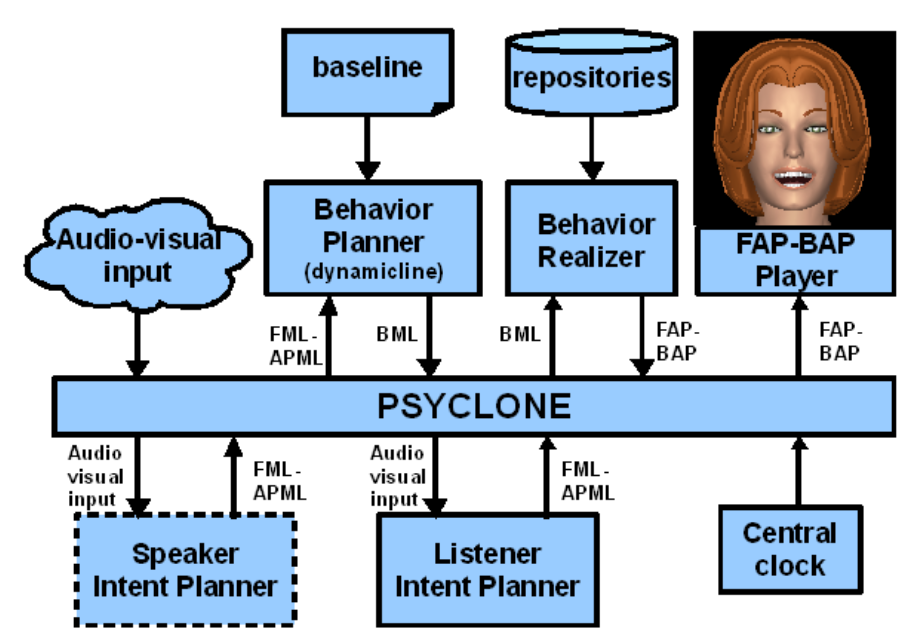
\includegraphics[width=0.6\textwidth]{images/GretaArchitecture.png}
	\caption{GRETA architecture. From~\cite{Niewiadomski2009}}
	\label{fig:GretaOriginal}
\end{figure}



% there are four main modules  that supports the rapport strategies:
%\begin{itemize}
%	\item \textbf{\ac{SSI}}: recognise social signals in realtime;
%	\item \textbf{SHORE}: recognise emotions from a video feed;
%	\item \textbf{GRETA\textsuperscript{PP}}: adapted version of GRETA~\cite{Niewiadomski2009} to generate listener behaviour;
%	\item \textbf{GRETA \textit{Perceiver} Plugin}: proxy between GRETA\textsuperscript{PP} and the \textit{Rapport Controller}.
%\end{itemize}


\subsection{Facial Expression Mimicry}
\label{sub:sec:FacialExpressionMimicry}

The Facial Expression Mimicry rapport \textit{Effector} mimics the user's emotion given the perceptual information returned from SHORE (the source code is available in listing~\ref{lst:facialExpressionsSourceCode} in Appendix C). The \textit{Effector}'s parameters (Table~\ref{table:facialMimicryParameters}) were attributed empirically following several pilots that were run with 3 different people until a balance was found between overeagerness and lack of liveness (Table~\ref{table:facialMimicryParametersValues}). In particular, the probability and the minimum delay specified in Table~\ref{table:facialMimicryParametersValues} were crucial to avoid triggering animations one, after another, for the duration of the emotion. In addition, the final \textit{Nutty Tracks} animation identifier is the base identifier followed by a random number between 1 and 5, for example, \textit{sadness1}, \textit{joy4}, and \textit{surprise3}. With this randomisation, the agent will not be as repetitive which may impact negatively the user's opinion of it. %Lastly, Anger is not specified as SHORE often mistakes it for happiness.

Nonetheless, the implementation of this plugin is not without issues as:
\begin{itemize}
    \item In absence of faces, SHORE outputs happiness emotions with a high level of intensity ($>$ 75);
    \item There is a slight noticeable delay (less than 1 second) between the emotion appearing on the video feed and being transmitted to GRETA;
    \item Camera distance and light conditions have the greatest impact on accuracy.
\end{itemize}

The issues lied on a balance between accuracy and speed. Applying a smoothing filter solved the second issue by reducing the signal spikes but it increased the delay from at most 1 second to 3 seconds. In the end, we opted to remove the smoothing filter, compensating with enabling/disabling this plugin only when required in runtime (Section~\ref{sub:sec:effectorPlugin}). Finally, the last issue is easily solved by taking the lightning conditions into consideration when preparing the physical space.

\begin{table}[H]
	\centering
	\begin{tabular}{|l|c|c|c|}
	\hline
	\multicolumn{1}{|c|}{\textbf{Parameter}} & \textbf{Happiness} & \textbf{Sadness} & \textbf{Surprise} \\ \hline
		Priority & 1 & 1 & 1 \\ \hline
		Minimum Intensity & 0.65 & 0.65 & 0.5 \\ \hline
		Trigger Probability & 0.48 & 0.48 & 0.48 \\ \thickhline
		\textit{Nutty Tracks} Base Animation & joy & sadness & surprise \\ \hline
		Minimum delay between mimicry behaviours (ms) & 3500 & 3500 & 3500 \\ \hline	
	\end{tabular}
	\caption{Parametrisation of the Facial Expression Mimicry rapport \textit{Effector}. }
	\label{table:facialMimicryParametersValues}
\end{table}


\subsection{Head Gesture Mimicry}
\label{sub:sec:HeadNodMimicry}

The Head Gesture Mimicry rapport \textit{Effector} mimics up-down nod gestures and left-right head shakes given the perceptual information returned from \ac{SSI}. In order to make \ac{EMYS} mimic head gestures, we added head nods and head shakes animations to \textit{Nutty Tracks} that takes into account the \textit{Effector} parameters specified in Table~\ref{table:headNodMimicryParameters}. The \textit{Effector} parameters were attributed empirically similar to Facial Expression Mimicry \textit{Effector} (Table~\ref{table:headGesturesMimicryParametersValues}), however, as the sensors seldom detected head gestures during the pilot tests, both gestures' probabilities were set to 1, that is, the agent will always mimic the behaviour.

Lastly, similarly to Facial Expression Mimicry \textit{Effector}, there is an apparent latency between the user's action and the mimicry behaviour, that is only solved by increasing the computational resources.

\begin{table}[H]
	\centering
	\begin{tabular}{|l|c|c|}
	\hline
	\multicolumn{1}{|c|}{\textbf{Parameter}} & \textbf{Up-Down Nods} & \textbf{Left-Right Shakes} \\ \hline
		Priority & 1 & 1 \\ \hline
		Trigger Probability & 1 & 1 \\ \hline
		Intensity Range ($I_{min}$, $I_{max}$) & (10,20) & (40,60) \\ \hline
		Repetitions Range ($R_{min}$, $R_{max}$) & (2,2) & (2,2)\\ \hline
		Frequency Range ($F_{min}$, $F_{max}$) &  (40,55) & (40,55)\\ \thickhline		
		Minimum delay between mimicry behaviours (ms) & 3500 & 3500 \\ \hline		
	\end{tabular}
	\caption{Parametrisation of the Head Gesture Mimicry rapport \textit{Effector}.}
	\label{table:headGesturesMimicryParametersValues}
\end{table}
\subsection{Mutual Gaze}
\label{sub:sec:GazeFace}

The Mutual-Gaze rapport \textit{Effector}, as described in Section~\ref{sec:mutual_attentionModel}, swaps the gaze target depending on the user's personality and on the current state of the interaction, more precisely, whenever the agent is in an in-task phase, or in a between-task phase. As we not know the personality of the user beforehand, the \textit{Effector} assumes that the interactional partner is extroverted (which has lower standard deviation than introvert following Table~\ref{table:gazetimes}). This \textit{Effector} plugin uses the rapport model's default durations parameters which are represented in Table~\ref{table:mutualGazeParametersValues}. Finally, the gaze targets identifiers depicted on the same table are known by \textit{Skene} who triggers the appropriate animations on \textit{Nutty Tracks}.

\begin{table}[H]
	\centering
	\begin{tabular}{|l|c|c|}
	\hline
	\multicolumn{2}{|c|}{\textbf{Parameter}} & \textbf{Value} \\ \hline
	\multicolumn{2}{|l|}{In-task Gaze Priority} & 1 \\ \hline
	\multicolumn{2}{|l|}{Between-tasks Gaze Priority} & 1 \\ \hline
	\multirow{2}{*}{In-task} & Face & 2660 \\ \cline{2-3} 
	 & Task & 4040 \\ \hline
	\multirow{2}{*}{Between-tasks} & Face & 3910 \\ \cline{2-3} 
	 & Task & 1010 \\ \thickhline
	\multicolumn{2}{|l|}{Face Gaze Target Identifier} & middleFront \\ \hline
	\multicolumn{2}{|l|}{Task Gaze Target Identifier} & bottomFront \\ \hline
	\end{tabular}
	\caption{Parametrisation of the Mutual Gaze rapport \textit{Effector}.}
	\label{table:mutualGazeParametersValues}
\end{table}

%Despite SHORE being capable of estimating accurately the gender of the user, it must be defined beforehand by the developer. 








%table:mutualGazeParameters
%table:backchannel
%table:headNodMimicryParameters


\subsection{Backchannel}
\label{sub:sec:backchannel}

The Backchannel rapport \textit{Effector} is based on the work developed on the GRETA system~\cite{Niewiadomski2009}, that analyses the variations of the pitch perceived by the openSMILE component of \ac{SSI}. Given the backchannel timings received from the GRETA\textsuperscript{PP} \textit{Perceiver} plugin, the \textit{Effector} plugin produces only head nods, as we were not able to generate a convincing \textit{Hmm hmmm} with a similar pitch as the generated voice by the \textit{Speech Server}. Ideally, the agent would alternate between head nods, \textit{Hmm hmmm} vocalisations, or both head nods and vocalisations. The parameters' values are depicted in Table~\ref{table:headGesturesMimicryParametersValues}, which are almost identical to the ones used in the Head Gesture Mimicry \textit{Effector}, except the priority is higher as the action proposals are executed on discrete states of the interaction. The trigger probability is identical to the one used in GRETA.

Despite succeeding with the integration of \ac{SSI} and GRETA, the resulting Backchannel \textit{Effector} did not behave as expected due to environmental factors that could not be controlled without changing the agent's embodiment as:
\begin{itemize}
	\item The \ac{EMYS}'s movement are noisy;
	\item The \ac{EMYS}'s voice is played through external speakers.
\end{itemize}

We attempted to reduce the impact of these factors by:
\begin{itemize}
	\item Use directional noise-suppressing microphone;
	\item Reduce the microphone sensivity;
	\item Adapt the \ac{SSI} pipeline to increase the pitch baseline.
\end{itemize}

To conclude, despite these efforts, this \textit{Effector} did not behave as intended, therefore it was not used in the user studies in Chapter~\ref{chap:userstudies}.

\begin{table}[H]
	\centering
	\begin{tabular}{|l|c|}
	\hline
	\multicolumn{1}{|c|}{\textbf{Parameter}} & \textbf{Backchannel Head Nod}\\ \hline
		Priority & 2 \\ \hline
		Trigger Probability & 0.4 \\ \hline
		Intensity Range ($I_{min}$, $I_{max}$) & (10,20) \\ \hline
		Repetitions Range ($R_{min}$, $R_{max}$) & (2,2) \\ \hline
		Frequency Range ($F_{min}$, $F_{max}$) &  (40,55) \\ \thickhline		
		Minimum delay between mimicry behaviours (ms) & 5000 \\ \hline		
	\end{tabular}
	\caption{Parametrisation of the Backchannel rapport \textit{Effector}.}
	\label{table:headGesturesMimicryParametersValues}
\end{table}

\section{Final Remarks}
During the previous sections, the document describes the system that implements the rapport model described in Chapter~\ref{chap:rapportModel} and extends the \ac{SERA} ecosystem to create robotic agents capable of managing rapport following current literature on models that tailor behavioural strategies to the dyadic state of the interaction. The presented \textit{Effectors} were developed and tested for robot \ac{EMYS} (Figure~\ref{fig:robots:EMYS2}), therefore the values described in Tables~\ref{table:facialMimicryParametersValues} to~\ref{table:headGesturesMimicryParametersValues} are tailored to this embodiment. Auxiliary plugins may have been developed by the researcher to monitor the scenario and trigger contextual utterances that will attempt to enhance positivity and build rapport.  In additional, the system aids the development of customisable plugins so that they can be easily changed by non-technical researchers such as psychiatrists whose knowledge on \ac{HRI} is crucial to building agents. Finally, and above all, pilot tests should be done so that the final set of possible actions sent by the agent are effective on satisfying the interactional goals of the scenario and manage rapport with the user.


%, and on the work developed by Huang et. al.~\ref{Buschmeier2011} on a virtual rapport agent. 
%Limited backchannel behaviours 


